\documentclass[draftclsnofoot, onecolumn, compsoc, 10pt]{IEEEtran}
\usepackage{lscape}
\usepackage{rotating}
\usepackage{titling}
\usepackage[margin=0.75in]{geometry}
\usepackage{graphicx}
% \usepackage{placeins}
\usepackage{caption}
% \usepackage{float}
\usepackage{url}
\usepackage{natbib}
\usepackage{setspace}
\usepackage[section]{placeins}
\graphicspath{ {images/} }
\linespread{1.0}
\parindent=0.0in
\parskip=0.2in
\geometry{textheight=9.5in, textwidth=7in}

\usepackage{listings}
\usepackage{color}

\definecolor{dkgreen}{rgb}{0,0.6,0}
\definecolor{gray}{rgb}{0.5,0.5,0.5}
\definecolor{mauve}{rgb}{0.58,0,0.82}

\lstset{frame=tb,
  language=Java,
  aboveskip=3mm,
  belowskip=3mm,
  showstringspaces=false,
  columns=flexible,
  basicstyle={\small\ttfamily},
  numbers=none,
  numberstyle=\tiny\color{gray},
  keywordstyle=\color{blue},
  commentstyle=\color{dkgreen},
  stringstyle=\color{mauve},
  breaklines=true,
  breakatwhitespace=true,
  tabsize=3
}



\title{\huge Spring Progress Report}
\author{Oregon State University\\CS 463\\2017-2018\\\\Prepared By:\\ Kyle Prouty\\Hayden Anderson\\}

\def \CapstoneTeamName{			Rodents Of Unusual Size}
\def \CapstoneTeamNumber{		46}
\def \GroupMemberOne{			Hayden Anderson}
\def \GroupMemberTwo{			Kyle Prouty}
\def \CapstoneProjectName{		Project ROUS}
\def \CapstoneSponsorCompany{	HP, Inc}
\def \CapstoneSponsorPerson{	Lonnie Mandigo}

\def \DocType{ Spring Progress Report }
			
\newcommand{\NameSigPair}[1]{\par
\makebox[2.75in][r]{#1} \hfil 	\makebox[3.25in]{\makebox[2.25in]{\hrulefill} \hfill		\makebox[.75in]{\hrulefill}}
\par\vspace{-12pt} \textit{\tiny\noindent
\makebox[2.75in]{} \hfil		\makebox[3.25in]{\makebox[2.25in][r]{Signature} \hfill	\makebox[.75in][r]{Date}}}}

\begin{document}
\begin{titlepage}
    \pagenumbering{gobble}
    \begin{singlespace}
        \hfill  
        \par\vspace{.2in}
        \centering
        \scshape{
            \huge CS Capstone \DocType \par
            {\large\today}\par
            \vspace{1in}
            \textbf{\Huge\CapstoneProjectName}\par
            \vspace{1in}
%             \vfill
%             {\large Prepared for}\par
%             \Huge \CapstoneSponsorCompany\par
%             \vspace{5pt}
%             {\Large\NameSigPair{\CapstoneSponsorPerson}\par}
            {\large Prepared by }\par
            Group\CapstoneTeamNumber\par
            \CapstoneTeamName\par 
            \vspace{5pt}
            {\Large
                \NameSigPair{\GroupMemberOne}\par
                \NameSigPair{\GroupMemberTwo}\par
            }
            \vspace{20pt}
        }
        \vfill
        \begin{abstract}
        \noindent 
        This document gives a Spring term update overview of the ROUS framework. To start we will go over the project's purpose and goals. Next we will go over the current progress and what we still have left to accomplish. Then we will discuss the problems encountered and how we worked through them. Finally, we will show some important code snippets and images that explain different features and aspects to the ROUS framework.

        
        \end{abstract}     
    \end{singlespace}
\end{titlepage}
\newpage
\pagenumbering{arabic}
\clearpage 
\tableofcontents
\pagebreak

%%%%%%%%%%%%%%%%%%%%%
% Report

% briefly recaps the project purposes and goals
% describes where you are currently on the project
% describes what you have left to do
% describes any problems that have impeded your progress, with any solutions you have
% includes particularly interesting pieces of code (if coding is involved)
% includes images of your project -- screen shots, photos, whatever is appropriate
% Clarity of thought, presentation, spelling, and grammar will all be evaluated for grading purposes. Please ensure you take this document seriously.
%%%%%%%%%%%%%%%%%%%%%%



\section{Project Overview}
\subsection{Purpose}
% OLD
% The framework being developed will create a network of nodes that will communicate by broadcasting simple messages to each other. Nodes will use network protocols to pass these messages in order to self organize on an objective. Users will be able to input print job objectives into our framework and view the results from a graphical user interface.

% Overall the rationale for the entire framework is to have a collection of loosely coupled nodes that can self organize to accomplish a print job. This framework will be robust in the face of any nodes that become untrusted. Nodes in this framework will communicate with each other using simple messages over wireless network protocols.

% \subsection{Framework Design}
% The ROUS framework being implemented will be organized into three parts: software, hardware, and a graphical user interface. These separate pieces will work together to make up the overall framework. This system will have the functionality to be given a print job objective, organize on that objective, and then accomplish that print job objective.

% In this framework all communication happens by broadcasting simple messages. A user interface will provide users, observers, and administrators the ability to interact with the framework. The framework will contain a network of nodes that communicate by broadcasting simple messages. 
% \begin{figure}[H]
% \centering
% 	\captionsetup{justification=centering}
%     \caption{This is a basic context view of the overall architecture of the ROUS framework}
% \end{figure}
% The Rodents Of Unusual Size (ROUS) framework aims to create a collection of loosely coupled nodes that will communicate and collaborate on user input objectives via simple broadcasted messages. This community of nodes are dynamic, self-sufficient, and secure. The goal of this communications framework will revolutionize the Internet of Things (IoT) technology. Users can input an objective into their Intranet and the community of social devices communicate on how to accomplish the service. 

\subsubsection{Problem}
The Internet of Things is growing larger everyday with millions of new devices coming online. These devices depend on reliable networks to communicate and make decisions. Without these stable networks these devices have no other method of communication.

\subsubsection{Solution}
To solve this problem, we have created a community of devices that can make social decisions in order to collaborate and accomplish an objective. The devices are stateless and can communicate without the need of a reliable network communication. Instead, these devices communicate directly with each other in order to make social decisions.

\subsection{Goals}

% There are a lot of end goals we have for our system. For the system to work as we intend, it shall:
We started development on this project with the following requirements in mind:
\begin{itemize}
\item Enable nodes to self organize on a structured objective
\item Allow an objective to be input
\item Allow a source of mistrust to be input
\item Output readable configuration data
\item Output readable system state data
\item Output readable results of objective
\item Automatically validate and connect to authorized nodes
\item Allow nodes to share objectives with each other
\item Framework state changes based on the input of a source of mistrust
\item Have a user interface
\item Offer a print service
\end{itemize}
In the end we were able to accomplish these requirements. We have created a community of nodes that can self organize on an objective. Nodes can work together to make a social decision. Each node offers a set of services and some nodes offer a print job service. The ROUS framework has a frontend interface that allows the user to input simple and complex services. Users can see the nodes bid on services, see who wins the service, and what service was won using our graphical interface. Then the user see the nodes go back to waiting. There is a console log and a block graph to clearly display the steps that each node is taking after a user inputs a service into the node network.

\section{Current Progress}
\subsection{Ongoing Work}
Overall we have completed all the requirements set out in our requirements document. Now we are just refactoring the project folder structure and cleaning up random spaces and print statements throughout the code. We are fixing bugs and working to make sure the code base is robust as possible for expo.
% We are currently refactoring a lot of our code to be more modular 
% and have similar code blocks to be organized with each other. 
Also, we are updating the user view of the GUI to match the new and improved administrator GUI. 

\subsection{What's Left}
Since we have already met our requirements for this project but still enjoy working on it, we are going to improve the system in both functionality and user experience. One objective we want to accomplish is to containerize our code with Docker. This will allow our framework to be ported to any operating system.
% OLD
% Over winter break and the ten weeks of winter term, most of our time will be spent on the development of our framework. Now that we have a clear view of the requirements and have set how the initial design should look, it is time to start implementation. Using the design document as a starting point, we will begin the process of coding and implementation. 
% To start the next step in the project, we will begin by laying out the code structure at a high level. We will write pseudo code and come up with the different pieces that need to be developed. From there we will start implementing the basic pieces of the framework, then work our way up to more complicated functionality. Overall, the next weeks and months will be spent implementing our first alpha level version of our framework.
% \subsection{Backlog}
% \begin{itemize}
% \item Be able to broadcast message
% \item Broadcast objective
% \item Language keywords
% \item Implement language
% \item Implement "and" in language
% \item Implement "or" in language
% \item Task bidding
% \item Declare bid winner
% \item Task bidding: ties \= rebid
% \item Task bidding: ties \= only top tied nodes rebid
% \item Carryout objective
% \item Node can print to a printer
% \item GUI base
% \item GUI shows network
% \item GUI insert gets file
% \item GUI can broadcast to network
% \item GUI for administrator
% \item GUI for observer
% \item GUI for user
% \item GUI can receive messages
% \end {itemize}



\section{Problems Encountered}
\subsection{Problems}
% OLD
% One of the big problems we had when starting the project was the ambiguity of it all. There was a lot left open for interpretation but this allowed us to create our own project in a sense. Because of this ambiguity, we had to take more time to interpret and create a problem that needed to be solved as well as how we could solve it without needing a doctorate's degree.

% Another large issue we faced for most of the term was group dynamics. We had some trouble getting everyone to communicate and contribute to each piece of the project on time and have usable input. Once this escalated we knew very quickly that regular group handling dynamics would not work.
We have encountered a fair amount of technical problems throughout this term. We had the problem of the console log on the GUI being overloaded with messages, finding a good way to show past states of the nodes, and getting the Raspberry Pi's to connect and print to printers.

\subsubsection{ConsoleLog}
One of our big problems we had was the general console log for all messages in the system was consistently overloading and filling up the screen as soon as any nodes were connected. The console would be filled with "whois" messages. The "whois" messages are messages within the system for the nodes to know who is currently active in the system and what they are capable of doing. It is by far the most common type of message within the system. 

\subsubsection{BlockGraph}
Another problem we had was how we were going to show past states of the nodes within the ROUS network. For demos, we wanted a system for our GUI to intuitively show the past and current states, what services the node offers, and when it wins the bid on services. We started off the term using a library called "Sparklines"; this library seemed to do what we wanted when reading what it was and what it did. Unfortunately, when we applied the library and tried to get it to work for our needs we found it had a lot of weird inconsistencies and was unreliable. We had to find another way to show the past and current states of our nodes. This led to doing something similar as what we wanted out of "Sparklines", but with a block graph that would show through time and steps whether the node was waiting, bidding, or had won the bid. The logic to this turned out to be more difficult than expected and we were having trouble displaying the state correctly due to the issue with the amount of messages coming in. 

\subsubsection{Printers}
A large problem we had this term that we were not expecting was connecting the nodes to the printers. We underestimated the time it would take and the reliableness for Raspberry Pi's to connect to the printers as well as reliably get the printers to print within a reasonable amount of time. There were some printers we stopped using because they refused to print even when the nodes were connected correctly. We also found that using Pycups for printing was very finicky and would only work sometimes with certain printers. The amount of uncertainty and lack of documentation with Raspberry Pi's and printers caused the troubleshooting time and the time needed to setup demos to rise by an order of magnitude of what we originally expected.  


\subsection{Solutions}
% In the face of these problems we had to be creative and steadfast to overcome them. Some of the problems encountered were originally expected to be fairly trivial to solve and could be put off until the more current issues were dealt with. 
% However trivial some issues may present themselves, we have found to fully investigate and give more time than expected to resolve the problems. 

To fix the issue with the over abundance of messages within the "ConsoleLog", we took a step back from the issue and decided which messages were truly needed for somebody watching the system. We asked ourselves, "Can we show the information these messages convey somewhere else in the GUI?" Eventually, we settled on filtering the "whois" messages that constantly flooded the console log. We needed to filter these messages 
% and make sure to not print that there was still a message.
% We found we had to filter some input from the nodes 
in order to better show the activity within the nodes. 

By filtering some of the incoming messages, it caused us to rethink how we were looking at the incoming messages. Rethinking how we were getting the messages allowed us to make the problem we were having with the main block graph more manageable. Using a block graph with three separate rows for the three separate states we wanted to see the nodes be in was the way to go. We used the X-axis as time. After several weeks we got this graph to show the individual node's state over time.

Finally, when dealing with the printer problem
% we really found that time and repeating as well as trying to print in different ways was the best course of action. 
we found that instead of using Pycups to do printing, we used the much more reliable system commands with the Local Printer (LP) commands given by CUPS. This allowed us to confidently print each time, and it gave us assurance that each node was connected to its paired printer. 

The CUPS remote server GUI turned out to be the best way to ensure that a printer was connected correctly to a node.
% Our best action to ensure that the printer was connected correctly was by using the nodes CUPS server configuration GUI.
This GUI allowed us to connect remotely and configure the node. Once a node was configured through the interface, we could then call the LP commands using Python. This turned out to be the most reliable way to setup a printer with a one-to-one relationship to a node.

% and configure the correct printer each time it was ona  new network or had a new IP address. We had to change the configurations because when there is a new IP address associated with the printer, CUPS sees the printer as being a completely different printer. So the best course of action was to reconfigure, and clear the print queue each time we set up the nodes with the printers.

% OLD
% To solve the issue of ambiguity, we were able to come up with some time to sit down with our client and talk about our strengths and what we were interested in. The sole requirement of being Internet of Things (IoT) based, we needed to find a problem that needed solving within that scope. After seeing news headlines everywhere over the last couple years and each of us having some interest in the security of both our private networks as well as what the future could hold in terms of security, we settled on a security aspect of IoT frameworks. From this point we came up with the idea of a "mistrusted" node. This is when the collection of nodes can no longer "trust" what one of the nodes is saying or doing and how they work around that to still complete the objective.

% After trying techniques that were taught by Ombuds and past life experiences on dealing with differences in a workplace setting, the group dynamic issues were not only persisting, but escalating. We went to our TA, we went to Ombuds, and we finally went to the professors. When things were still escalating further, we went to our college of EECS advisor to get more advice since it was affecting our other classes as well. This problem was resolved by our professors and their solutions have cleared up the issues. 


\section{Code}
% Set language to Python
\lstset{language=Python}
\subsection{Node}
\subsubsection{Configuration}
\begin{lstlisting}
;[example]
;file: module_path
;function_in_module: %(file)s

[default]
file: utils/services.py
green_on: %(file)s
blue_on: %(file)s
pink_on: %(file)s
yellow_on: %(file)s
white_on: %(file)s
print_color: %(file)s
complex: %(file)s
\end{lstlisting}
The above code segment looks kind of boring but it is actually really powerful. Each node gets a configuration file, like the one above, and in that file is where the services that the nodes offer is defined. What is cool is that now a user does not have to go into the source code to add a new service. Instead, users can just create a a new Python module, and in that module have functions that will run a service. In the configuration file the user would only need to point to the module that contains all the service functions they defined, and then for each service function put a definition in the configuration like demonstrated above you have added a service.
% The above code segment shows what a typical configuration file looks like on a node. Using this modular setup allows future developers to create their own simple services for their devices and point to the user's new function definitions for their custom needs. 


\subsubsection{Multicast}
\begin{lstlisting}
#
def start_multicast_receiver(address):
	server_address = ('', mcast_port)
	sock = socket.socket(socket.AF_INET, socket.SOCK_DGRAM)
	sock.bind(server_address)
	sock.setsockopt(socket.IPPROTO_IP, 
                    socket.IP_ADD_MEMBERSHIP, 
                    struct.pack('4sL', socket.inet_aton(mcast_host), socket.INADDR_ANY))
	return sock

#
def send_multicast_message(message, key, address):
	try:
		multicast_group = (mcast_host, mcast_port)
		sock = socket.socket(socket.AF_INET, socket.SOCK_DGRAM)
		sock.setsockopt(socket.IPPROTO_IP, 
						socket.IP_MULTICAST_TTL, 
						struct.pack('b', 1)
						)
		encrypt_message = encryption.encrypt(str(message), key)
		sent = sock.sendto(encrypt_message, multicast_group)
		sock.close()		
	except:
		log.error("%s - FAILED to send: %s", address, message)
\end{lstlisting}
The code above is pretty boilerplate multicast code for python using underlying c sockets. I highlight this code because all the nodes and the user nodes use this same code to listen and send simple messages back and forth to each other. This code sits in a "utils" directory that both the nodes and user nodes use. This allows us to not have to repeat code and eliminates bugs because everyone is using the same mechanism.
% The above code snippet shows one way to print to the node's connected printer via Pycups. 
%the above code is definitely not worth showing

\subsection{Backend}
\subsubsection{Web Sockets and Trust}
\begin{lstlisting}
@io.on('trust')
def remove_trust(block_ip):
	find_nodes()
	newkey = str(encryption.newkey())
	removed.append(block_ip)
	if block_ip == str(0): #restore keys to all
		network.send_tcp_message(self_ip,"key,ukey,"+newkey)
		utils.write_new_key(utils.ukey(),newkey,self_ip)
		try:
			 for r in removed:
			 	if r != str(0):
			 		network.send_tcp_message(r,"key,ukey,"+newkey)
		except: pass
		if nodes:
			for n in nodes:
				node_ip = json.loads(n)['address']
				network.send_tcp_message(node_ip,"key,ukey,"+newkey)
	elif nodes: #remove key for selected node
		if block_ip != self_ip: #issues new key to myself
			network.send_tcp_message(self_ip,"key,ukey,"+newkey)
		for n in nodes: #issue new keys to all nodes but untrusted
			node_ip = json.loads(n)['address']
			print node_ip
			if block_ip != node_ip:
				network.send_tcp_message(node_ip,"key,ukey,"+newkey)
				utils.write_new_key(utils.ukey(),newkey,self_ip)

\end{lstlisting}
The function above is a little complicated and messy looking but it is pretty straightforward and demonstrates many different features in our framework. Overall this block of code just takes in an IP address to block and issues out new keys to all the nodes except the IP that was untrusted. It can also send out new keys to all nodes in the case of a reset. This code is interesting because it shows the use of both websockets and tcp. 

At the top of the function you can see "@io.on('trust')" which means that the when the frontend emits a "trust" message over websockets, the backend can then hear that message and then execute the below function. You can also see that this function uses a tcp server to send out the new encryption keys. We did not want to issue new keys via multicast so we setup a stateful connection with each node just to transfer the new key. 

% The above code segment shows the thread for the back end of the user node to continuously listen for messages within the system. Each message coming into the system to show the the state of the node that sent the message.

% % MAY END UP NOT PUTTING THIS IN, JUST THOUGHT IT WAS A GOOD INTERESTING PART OF CODE

\subsubsection{Messages}
\begin{lstlisting}
def find_nodes():
	network.send_multicast_message(
		'{"tag":"whois","address":"'+self_ip+'"}',ukey,self_ip)
	mutex.acquire()
	try:
		del nodes[:]
		if data:
			for d in data:
				d = json.loads(d)
				if d['tag'] == "info" and d['message'] == "whois":
					if nodes:
						check = False
						for n in nodes:
							n = json.loads(n)
							if str(d['address']) == str(n['address']):
								check = True
								break
						if not check:
							nodes.append(json.dumps(d))
					else:
						nodes.append(json.dumps(d))
	except:
		pass
	finally:
		del data[:]
		del console_data[:]
		mutex.release()
\end{lstlisting}
The function above is a good example of our systems use of simple message sending using JSON encoded strings. At the top of the function you can see that we are sending a simple JSON encoded string that can then be parsed out for its different parameters like "tag" or "message". Later in the function you can see us doing that. We can load in the raw string as a JSON object and then get the parameters that we want in order to filter out the correct data; in this case we are looking for nodes and then appending them to our data list.

\subsection{Frontend}
% Set language to Java because lstset does not support JavaScript as a language
\lstset{language=Java}
\subsubsection{Block Graph Logic}
\begin{lstlisting}
graphLogic = (graph,x,track,color) => {
    try{
      var check = false;
      track.map((data,i)=>{
        if(i===this.state.row.length-1 && data===2 && check===false){
          graph[i] = <td style={{backgroundColor:color}}/>
          this.clearGraph(track,x)
          check = true;
        }
        else if(data===1 && check===false){
          this.updateGraph(graph,track,i,color);     
          check = true;
          track[i] = 2;
        }
     });
    }finally{}
  };
  updateGraph = (data,track,i,color) => {
    data[i] = <td style={{backgroundColor:color}}/>;
    track[i] = 2;
    data.map((r,j) => {
      if(j > i)
        data[j] = <td style={{backgroundColor:""}}/>
    });
  };
  clearGraph = (track, x) => {
    this.state.track[x].map((t,i)=>{
      this.state.row_A[x][i] = <td style={{backgroundColor:""}}/>
      this.state.row_B[x][i] = <td style={{backgroundColor:""}}/>
      this.state.row_C[x][i] = <td style={{backgroundColor:""}}/>
      track[i] = 1
    });
  };
\end{lstlisting}
Above is some of the logic needed to accomplish the block graph. Getting the block graph to work took a lot of time and testing. Since we are only getting data by listening to simple messages, and the frontend knows nothing about the node network other then those messages. The little knowledge the frontend receives meant that building the GUI dynamically was more challenging. 

This block graph is interesting because it is built completely dynamically when new nodes are added or subtracted, for each node. Also, the block graph consists of a 3x3 array that has to correspond independently to each node that gets dynamically added. Adding more confusion is that we use only one block per each row between the three rows. Meaning that even though there are three rows, we need to think about it as having only a single row since only one of the three rows can be occupied for each column at a time. In the end the block graph is working stable and demonstrates what we set out for it to demonstrate to our users.

%  in the center of our administyrator GUI. Each node has a graph with three rows. The rows are separated for whether the node is waiting, bidding on a service, and if they won a service the node bid on. When one box in the rows gets filled, the other rows need to recognize and move to filling the next box if they are going to be the next to be filled.  

\subsubsection{ConsoleLog Filtering}
\begin{lstlisting}
filterTag = (data) => {
    if(JSON.parse(data)['tag']==="winner")
      return  <p style={{color:"green",fontWeight:"bold"}}>
                WINNER
                <p style={{fontWeight:"bold",color:"black"}}>
                  <div className="text-center" style={{marginLeft:"8%"}}>
                    {JSON.parse(data)['service']}</div>
                </p>
              </p>
    else if(JSON.parse(data)['tag']==="bidding")
      return <p style={{color:"red",fontWeight:"bold"}}>BIDDING</p>
    else if(JSON.parse(data)['tag']==="waiting")
      return <p style={{color:"blue",fontWeight:"bold"}}>WAITING</p>
    else
      return ""
  };
  consoleOutput = (data) => {
    if ((this.filterTag(data)) === ""){
      return
    }
    else {
      return ([
        <h4 style={{fontWeight:"bold",color:"#D73F09"}}>
          {this.filterAddress(data)}
        </h4>,
          this.filterTag(data),
      ])   
    }
  }
\end{lstlisting}
The code above is a good example of how we are filtering out unwanted messages before we display data on the "ConsoleLog" GUI component. Since the backend server is grabbing every message it hears and sending it to the frontend, the frontend must then do some filtering so that it does not display too much information and make the output confusing. In the code above you can see that data comes into the "consoleOutput" function, messages then get filtered by the tag and by the address. Having data as a string that can be encoded as JSON objects makes filtering out this data much more straightforward.

\newpage
\section{Project Images}
\begin{figure}[!htb]
\centering
	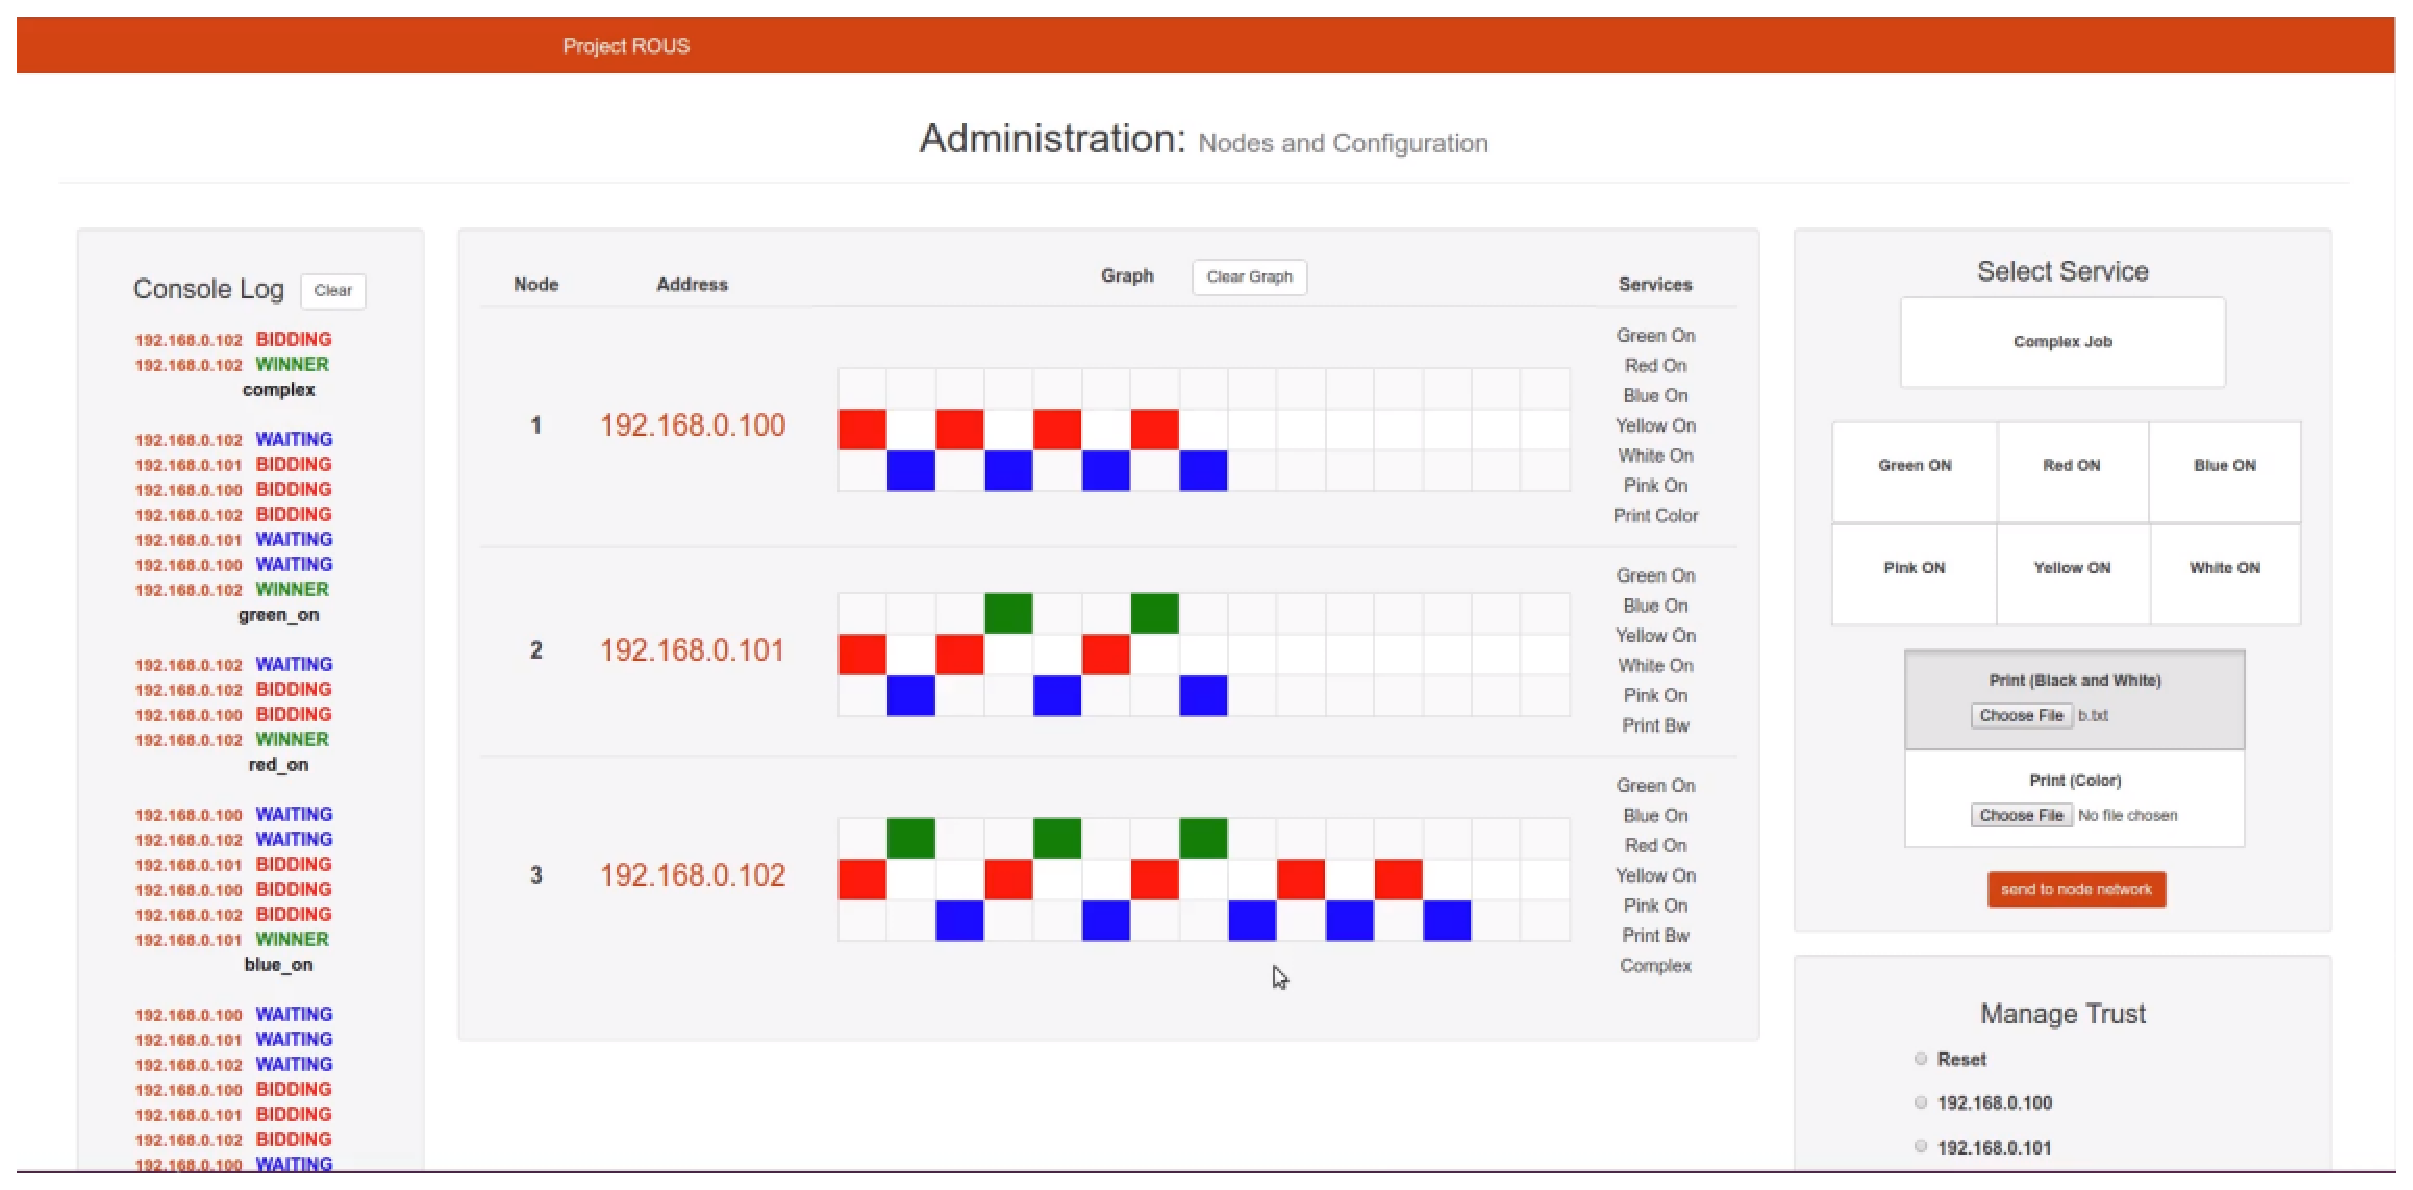
\includegraphics[width=1.0\textwidth]{img1}
	\caption{This is an image showing the frontend administrator user interface. You can see the result of three nodes socially collaborating on a complex service.}
\end{figure}
\begin{figure}[!htb]
\centering
	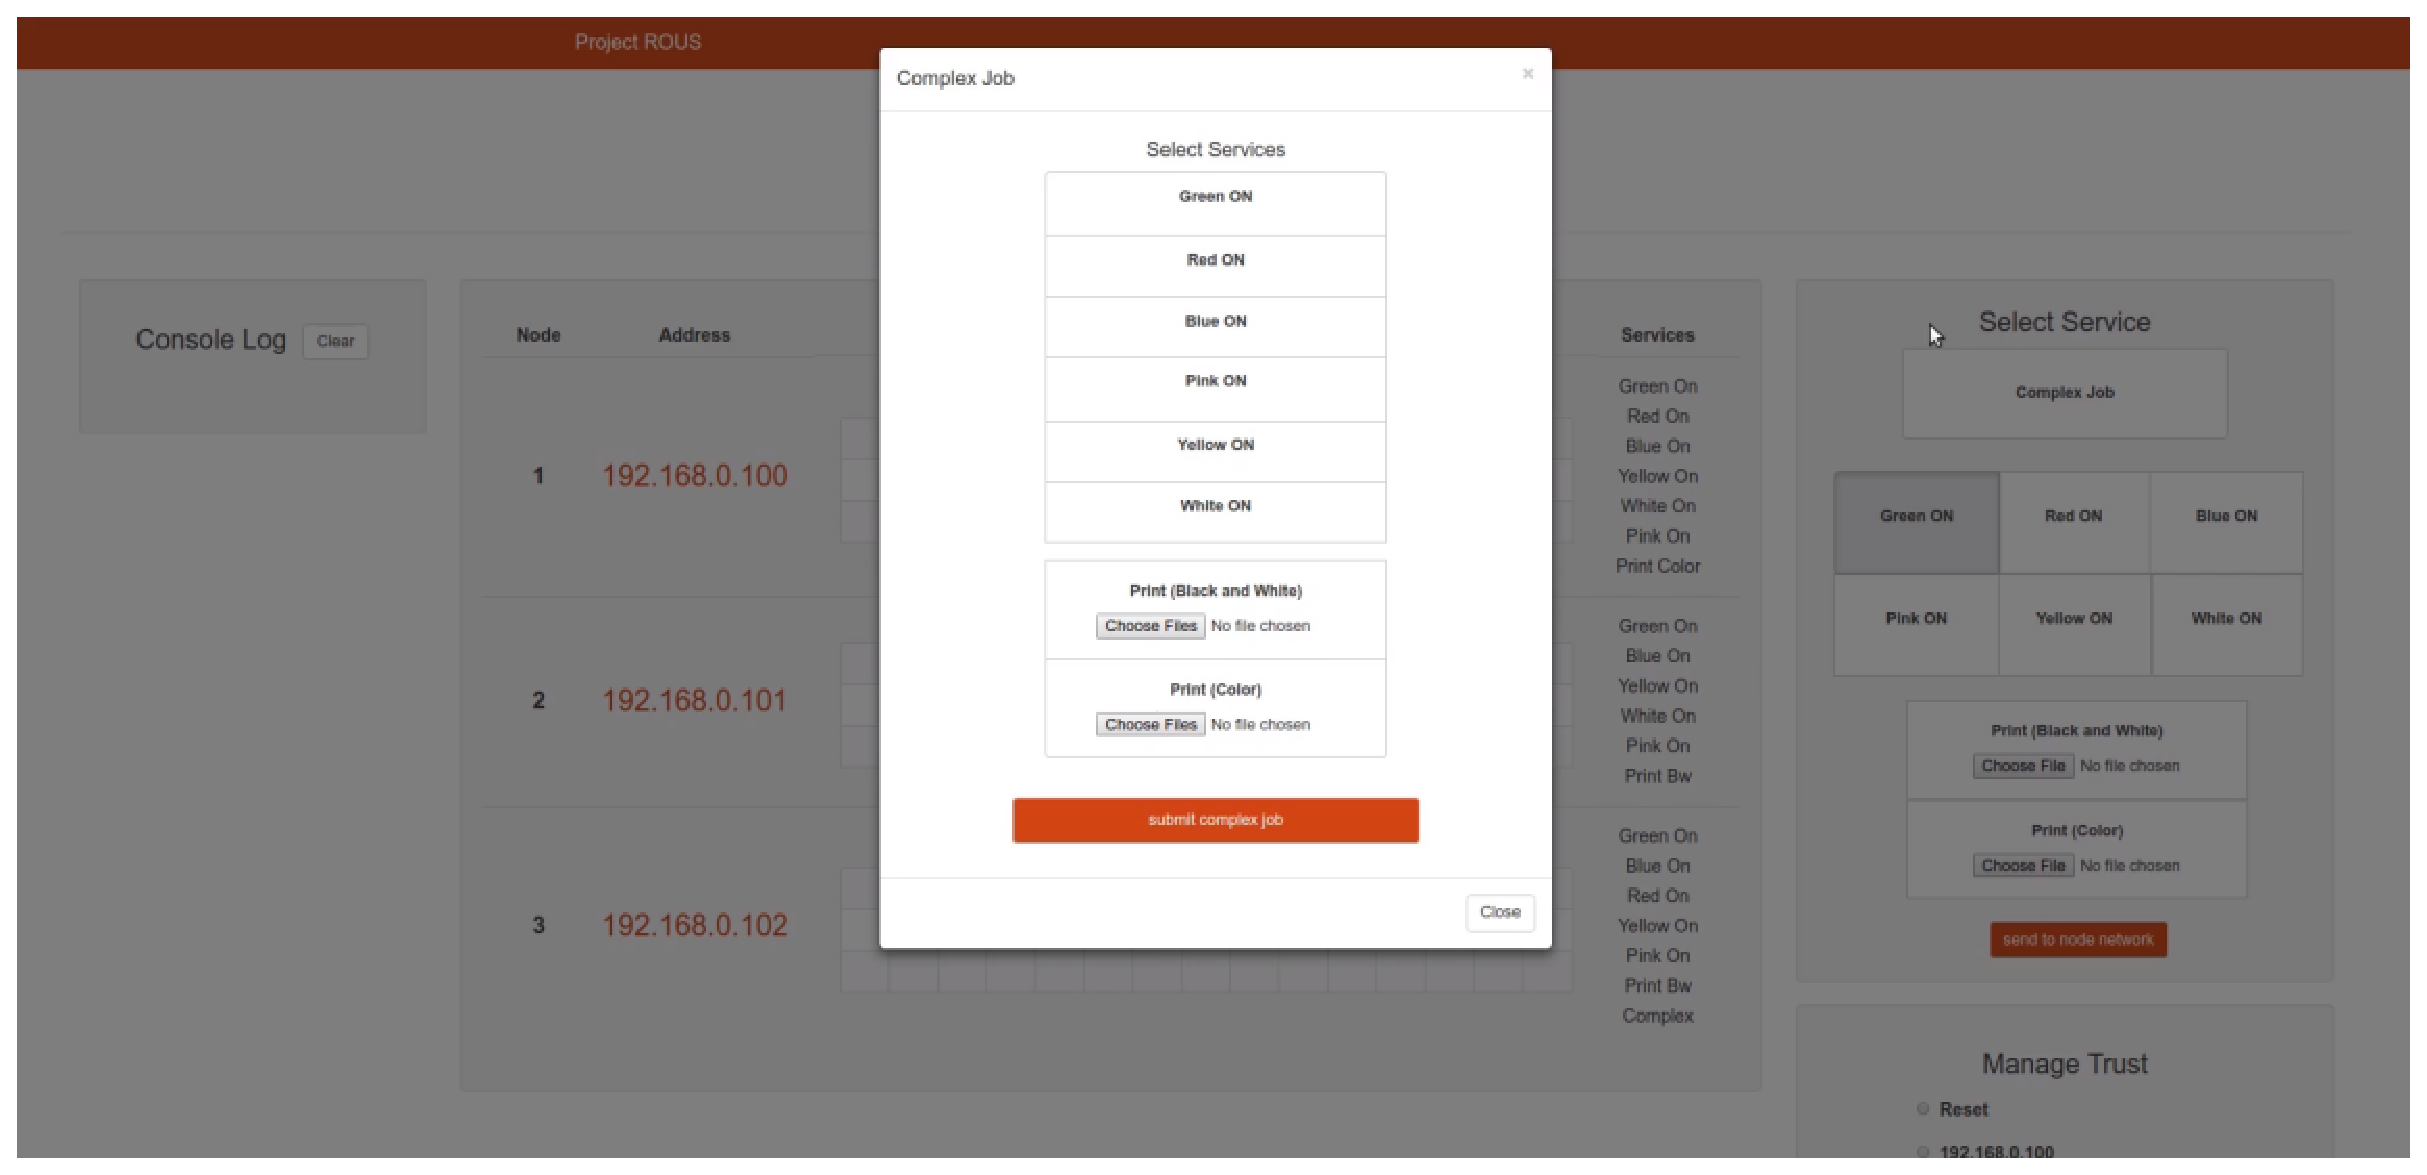
\includegraphics[width=1.0\textwidth]{img2}
	\caption{Showing the pop up modal on the administrator user interface that allows the user to input multiple services using a complex service.}
\end{figure}
\begin{figure}[!htb]
\centering
	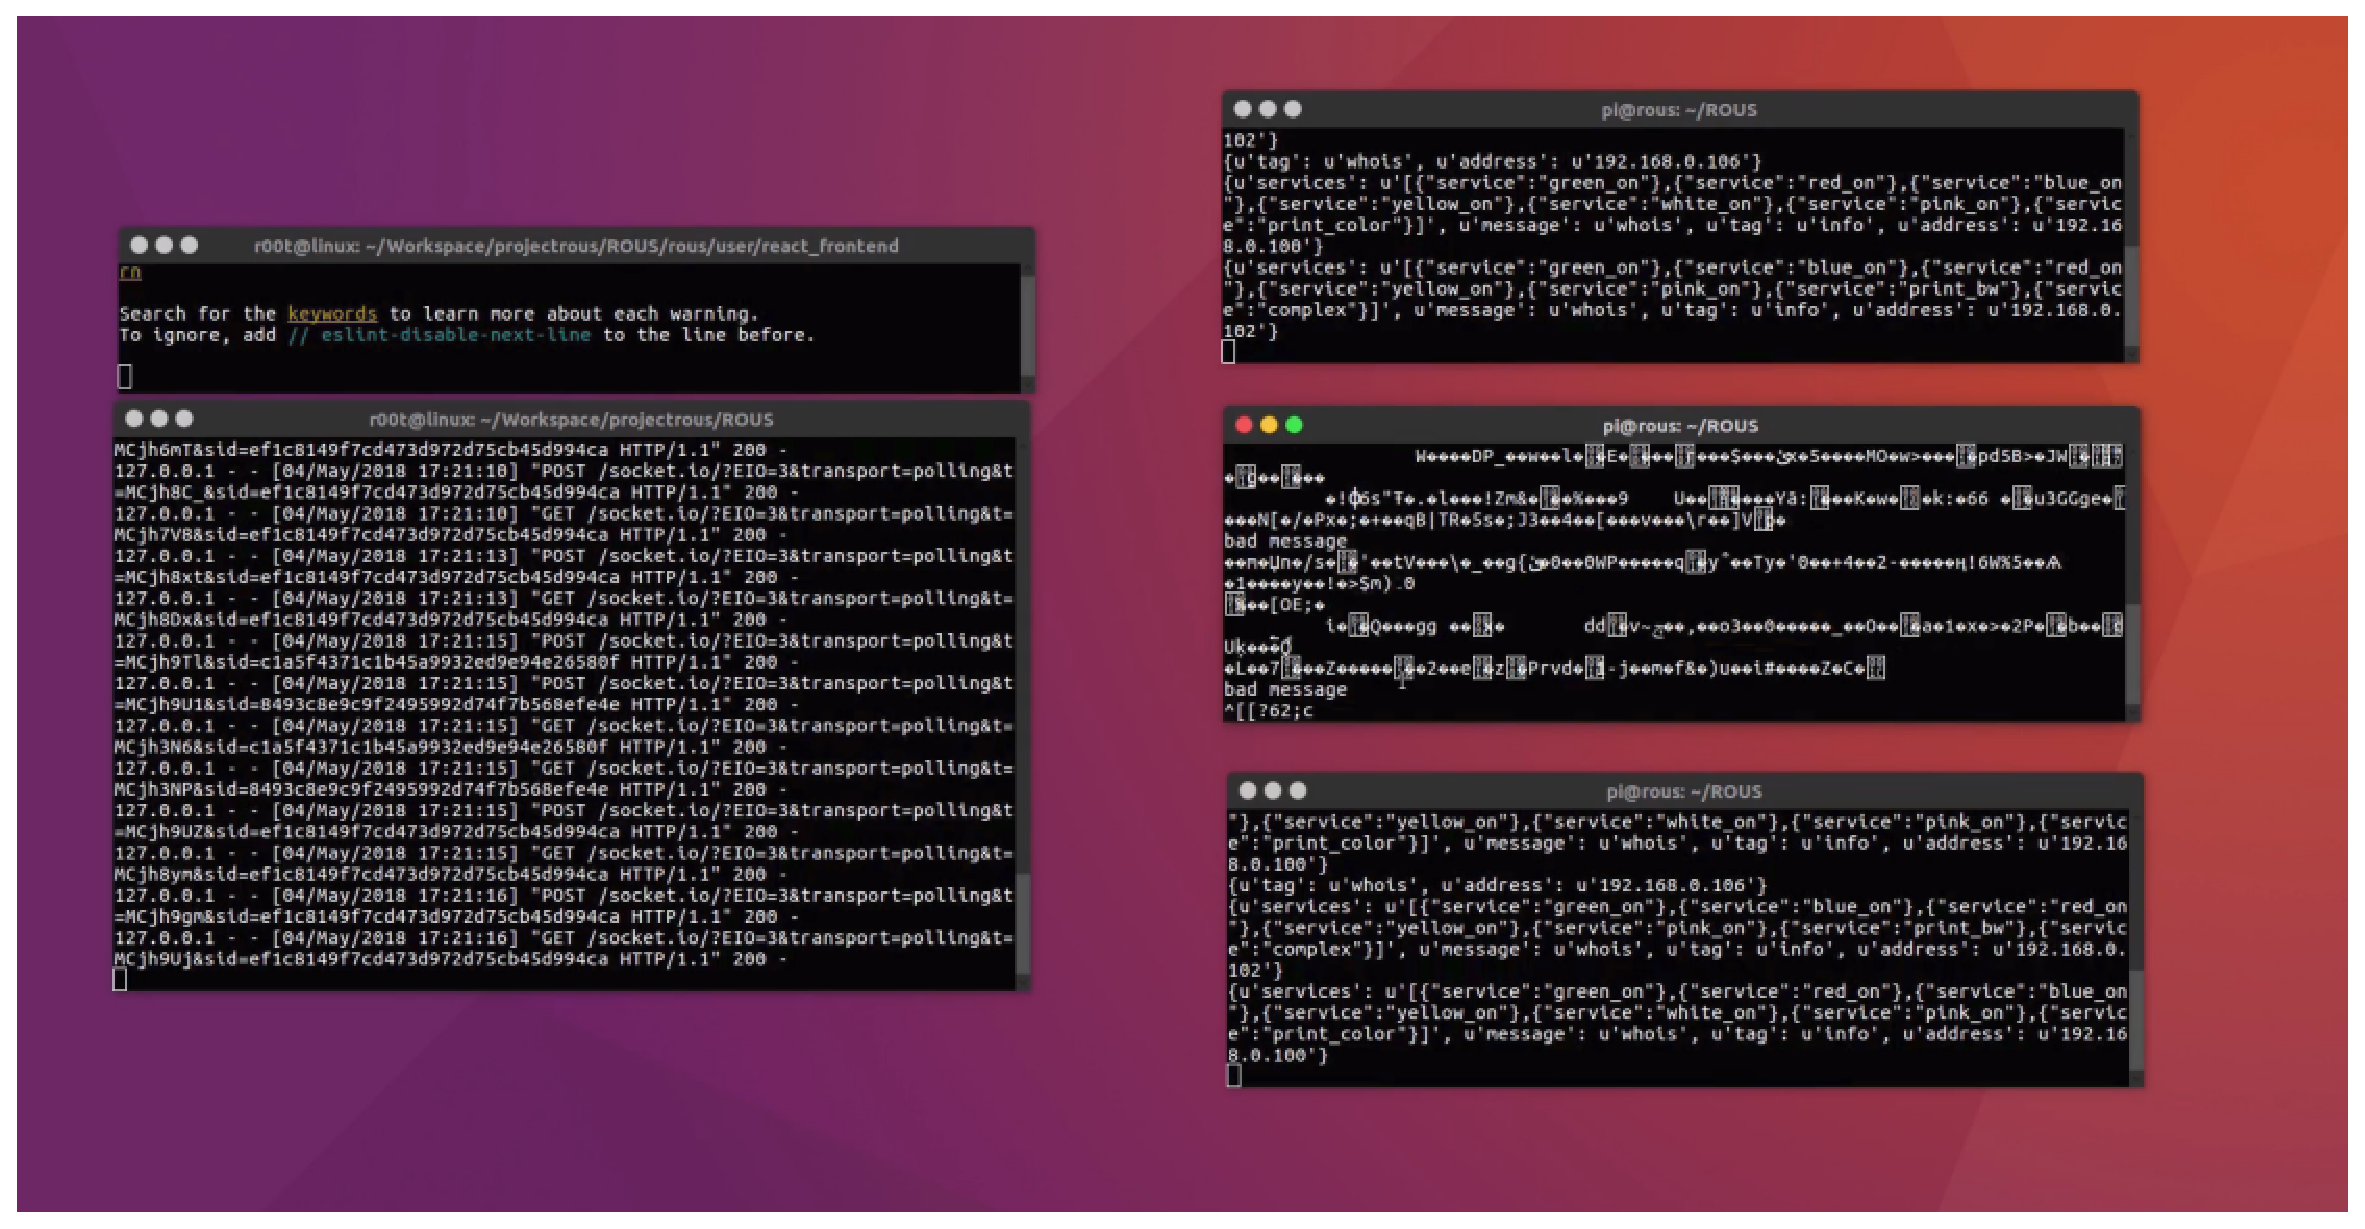
\includegraphics[width=1.0\textwidth]{img3}
	\caption{On the right hand side shows the command line shells that are running the frontend(top) and backend(bottom) programs that make up the user node. The left hand side shows three command line shells that represent the three nodes in our node network. In each shell we are ssh into each node and are running the ROUS framework node program. The middle node shows what happens when a node becomes untrusted and the garbage messages that it produces.}
\end{figure}
\begin{figure}[!htb]
\centering
	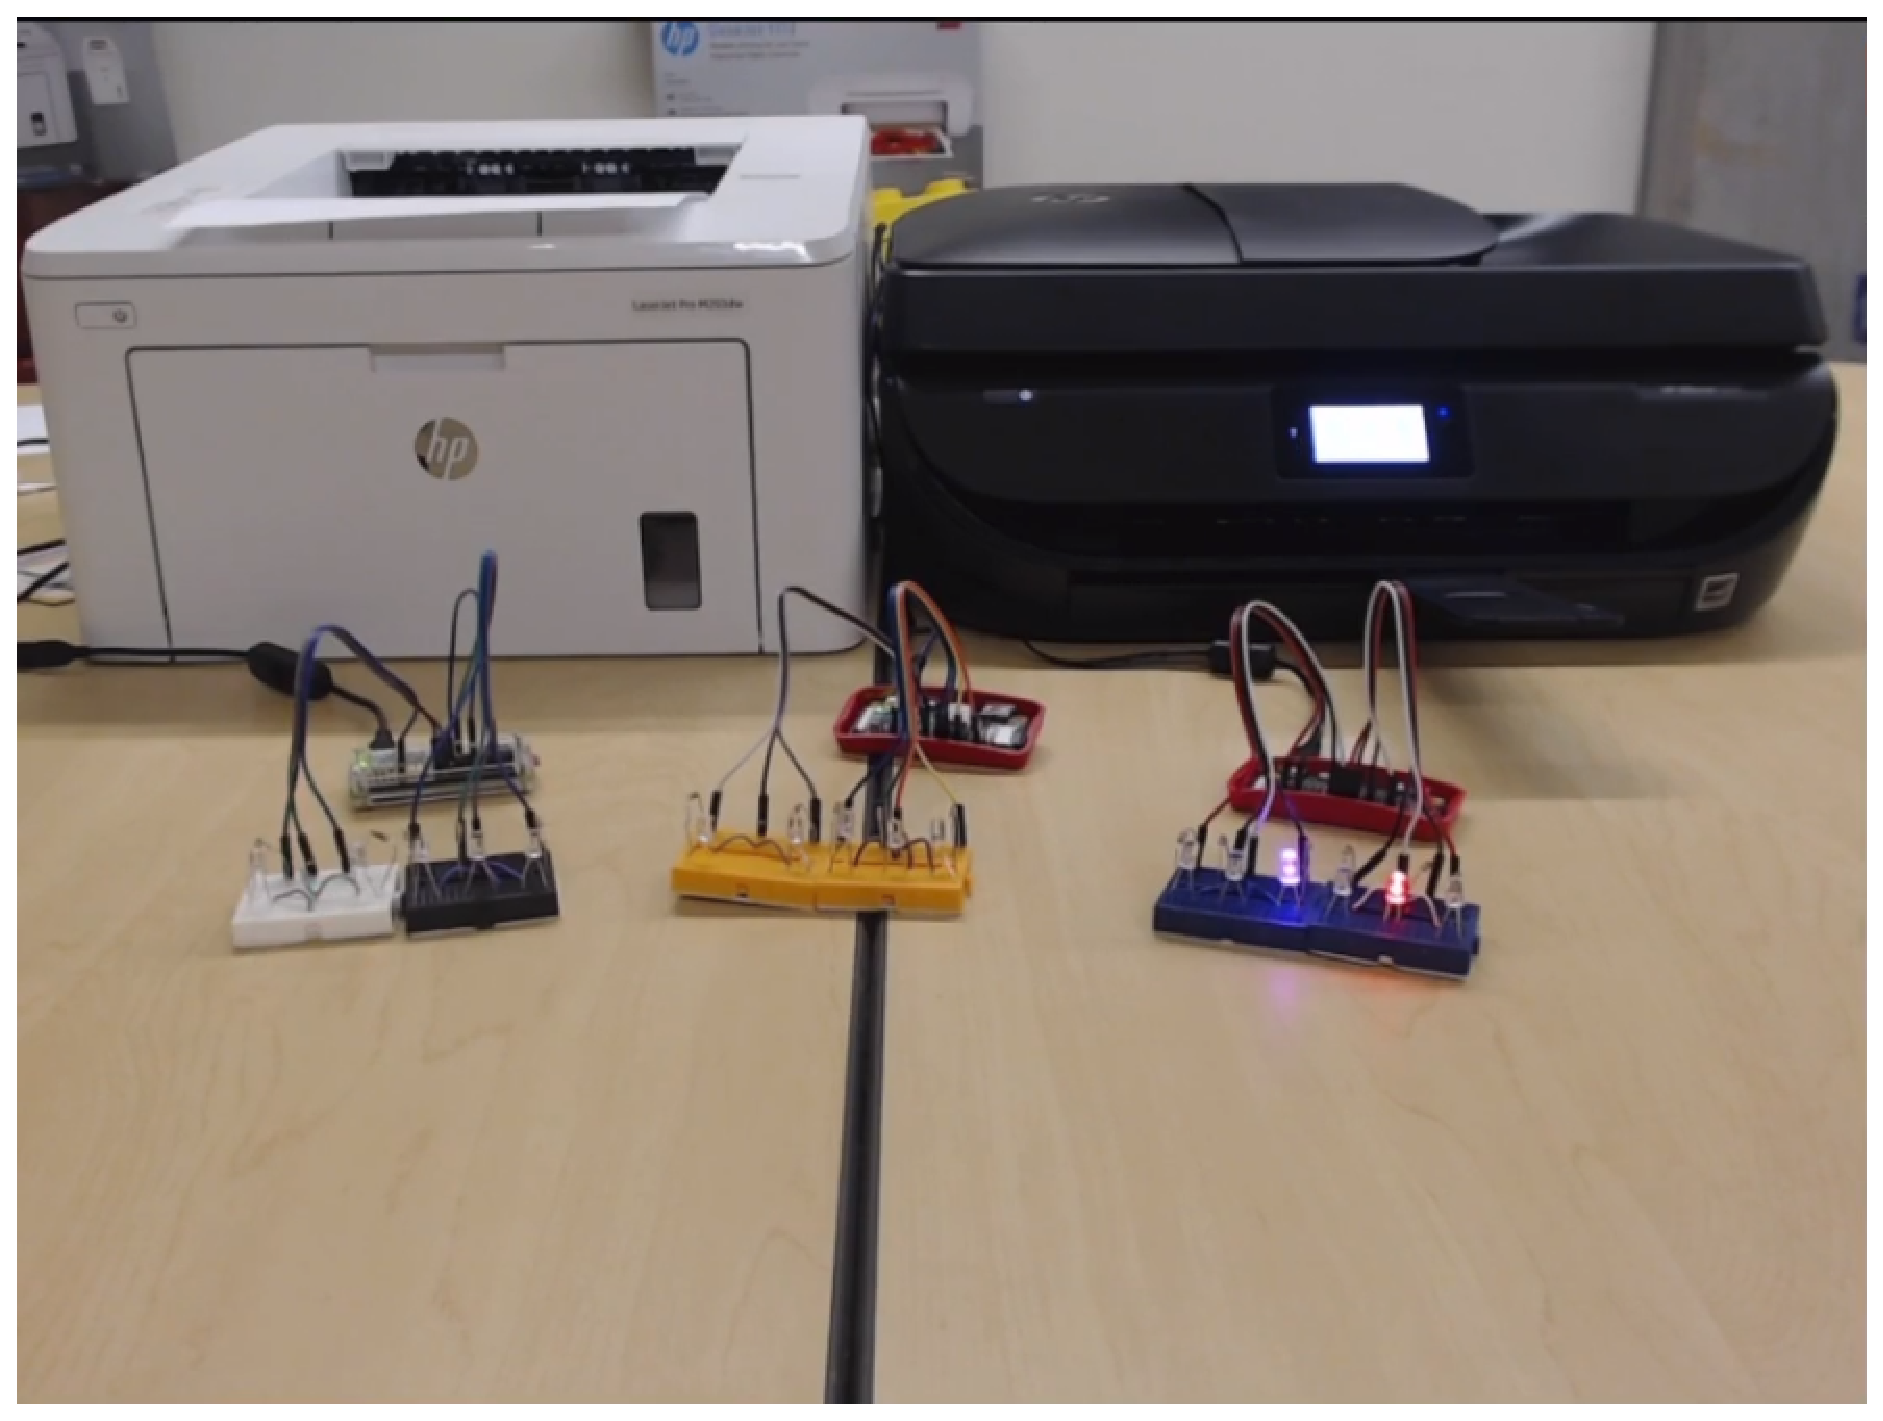
\includegraphics[width=0.7\textwidth]{setup}
	\caption{Showing the ROUS framework setup with three nodes and two printers. Each node is connected to a bunch of LEDs that represent services. Two of the nodes are connected in a one to one relationship with the two printers. The image shows the result of sending a pink on and red on service into the node network.}
\end{figure}

\section{Overall Summary}
We set out to create a community of devices that could make social decisions in order to collaborate and accomplish an objective. We wanted these devices to be stateless and communicate without the need of reliable network communication. Instead, these devices would communicate directly with each other in order to make social decisions.

% Throughout the course of this term we have had the opportunity to enhance the user's experience with our project in order to be able to demo and show off the ROUS framework. 
Through hard work and determination, we completed all of the requirements for our project, and even some of the stretch goals. We would still like to containerize our project using Docker to make distribution more straightforward for users. 

Overall, we have faced problems and kinks and spent a lot of this term troubleshooting and working through various bugs. In the end we have accomplished all the goals and requirements that we set out to accomplish and we will spend the remaining days before expo improving and polishing the framework.
% in the system we did not know we had until we were trying to show off our system. This term has been full of troubleshooting, whether it be the system to try and show off what is happening to the user or the printers and getting them to reliably connect and print with automated scripts. We have also found many solutions to our problems and were able to implement them successfully. We have a positive outlook on these coming weeks and plan on spending them improving the user experience and hammering down our project's "story" in order to explain what the ROUS system does to all walks of life; both technically minded and those less technically inclined.  

% OLD
% Over the course of fall term our team has made a lot of progress on the project. We have developed a problem statement, finalized the project's requirements, looked at relevant technologies that could be used to implement the project, and finally, discussed in detail how are project is designed. 

% We started this term very positive with a lot of motivation for the project. As the first few weeks progressed some group dynamics started to hurt the overall moral of the group. Eventually these issues were resolved. After the issues that plagued the first part of the term were dealt with, the rest of the term went smoothly. Both teammates, Hayden and Kyle, worked together well and communicated to accomplish the papers assigned. We developed a good relationship with our client, Lonnie, and communicate regularly. Our client provides us with excellent feedback which has helped us to improve our work.

% Despite the group dynamic issues faced throughout the term, our team was able to overcome persistent issues and work together to have a positive outcome. We worked hard to complete all work assigned and look forward to implementing the framework our the coming weeks and months.





\end{document}